% Local IspellDict: english

\documentclass[a4paper,12pt,twoside]{article}
\usepackage[english]{babel}
\usepackage{graphicx}
\usepackage{listings}

\lstset{
	language=ada,
	basicstyle=\footnotesize,
	numbers=left,
	numberstyle=\footnotesize,
	stepnumber=2,
	numbersep=5pt,
	showspaces=false,
	showstringspaces=false,
	showtabs=false,
	tabsize=2,
	captionpos=b,
	breaklines=true,
	breakatwhitespace=false
}
	
\widowpenalty=10000
\clubpenalty=10000

\begin{document}
\noindent\parbox[t]{9cm}{\textsf{Course 02158 Concurrent Programming\\
Fall 2011, DTU Informatics }}
\hfill
\parbox[t]{1cm}{\mbox{}\\
\raisebox{0.0cm}[1cm][1cm]{
\includegraphics[origin=lb]{dtu_logo_cmyk.pdf}}}

\vspace{2cm}

\begin{center}
{\Large \bf Solution to the mandatory assignment}\\
\vspace{0.3cm}
{\it Due Date : 16/11/2011}\\
\vspace{1cm}
{\Large Group 19}\\
\vspace{0.3cm}
\begin{tabular}{ccc}
{\large Jakub Judas}&{\large Nicolas Silva}&{\large Robin Del\'earde}\\
s110845&s111781&s111873
\end{tabular}\\
\end{center}

\newpage

\section{Introduction: the cars control problem}




\section{Step 3: the Barrier}
The purpose of this step is to implement a barrier on the playground in order to prevent the cars from making more rounds than the others. This is done by making every car stop at a barrier line, and wait for all the others before starting a new round. This synchronization issue can be solved with semaphores, which make it possible to check if all the cars are present at the barrier, and to make them wait while that's not the case, since a car is nothing more than a thread.\\
In order to stop those Car-threads, each car is assigned a semaphore, whose value is 0 while the car is not allowed to pass the barrier (the starting value is 0), and 1 either, thanks to a V operation triggered by the last car awaited. Those 9 semaphores are stored in a table called \textbf{barrier}.

\begin{figure}[h]
   \caption{\label{Barrier} crossing the barrier}
   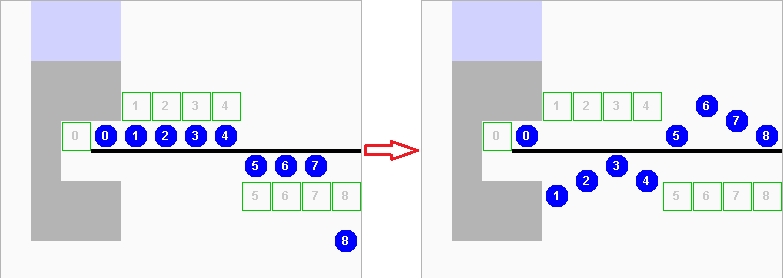
\includegraphics[width=14cm]{screens/Barrier}
\end{figure}

A barrier is defined by the Barrier class as:
\begin{itemize}
\item a table of 9 semaphores as described previously;
\item a boolean \textbf{ison} to control the state of the barrier;
\item a semaphore \textbf{access} and a boolean \textbf{pass}, used in the method \textit{sync} responsible for the access control at the barrier.
\end{itemize}
Actually this last semaphore acts as a counter allowing 7 cars to pass (the initial value is 7) and stopping the 8th one. Associated with the boolean \textbf{pass} whose value tells us where a car has been stopped in the program (i.e. by which semaphore: its own or the \textbf{access} one), it allows us to know when there's only one car left running on the playground. Then this car can release all the others when it arrives at the barrier.\\
The code of the synchronization class is given below, where \textbf{no} is the number of the car reaching this step:
\begin{verbatim}
public void sync(int no) {
   if (!pass) {
	   pass = true;
	   //only 7 cars may access this zone, the 8th one is stopped here
	   try { access.P(); } catch (InterruptedException e) {}
	   pass = false;
	   //the cars are stopped by the barrier
	   try { barrier[no].P(); } catch (InterruptedException e) {}
   }
   //the last car may pass here and releases everyone
   else {
	   pass = false;
	   for (int i=0; i<9; i++) {
		   if (i!=no) {
			   access.V();
			   barrier[i].V();
		   }
	   }
   }
}
\end{verbatim}


\end{document}